%----------------------------------------------------------------------------------------
%	PACKAGES AND THEMES
%----------------------------------------------------------------------------------------
\documentclass[aspectratio=169,xcolor=dvipsnames]{beamer}
\usetheme{Simple}

\usepackage{hyperref}
\hypersetup{
    colorlinks,
    linkcolor=black, % Overview
    urlcolor=blue    % \href#2
}

\usepackage{graphicx} % Allows including images

% colors
\usepackage{color}
\definecolor{black}{gray}{0}
\definecolor{g40}{gray}{.40}
\definecolor{g90}{gray}{.90}
\definecolor{r1}{rgb}{.75, .10, .10}
\definecolor{r2}{rgb}{.98, .01, .01}
\definecolor{r3}{rgb}{.99, .20, .40}
\definecolor{b1}{rgb}{.10, .10, .75}
\definecolor{b2}{rgb}{.16, .66, .97}
\definecolor{b3}{rgb}{.90, .90, .99}
\definecolor{b4}{rgb}{.00, .10, .60}
\definecolor{cy}{rgb}{.10, .70, .75}
\definecolor{g1}{rgb}{0.0, 1.0, .30}
\definecolor{g2}{rgb}{0.0, .60, .20}
\definecolor{g3}{rgb}{.05, .65, .05}
\definecolor{y1}{rgb}{.85, .50, .30}
\definecolor{y2}{rgb}{.99, .96, .60}
\definecolor{o1}{rgb}{.99, .80, .20}
\definecolor{o2}{rgb}{.99, .60, .30}

\newcommand{\red}{\color{r1}}
\newcommand{\blue}{\color{b1}}
\newcommand{\green}{\color{g3}}
\newcommand{\black}{\color{black}}
\newcommand{\cyan}{\color{cy}} % d2 f4 e5


% ding
\usepackage{fancybox}
\usepackage{pifont}
\def\Dstar{\ding{93}}
\def\Dsquare{\ding{114}}
\def\Dok{\ding{52}}
\def\Dko{\ding{56}}
\def\Dhand{\ding{42}}
\def\Dpen{\ding{47}}
\def\Darrow{\ding{220}}

%----------------------------------------------------------------------------------------
%	Macros
%----------------------------------------------------------------------------------------
\newcommand{\bi}{\begin{itemize}}
\newcommand{\ei}{\end{itemize}}
\newcommand{\param}[1]{{$\langle#1\rangle$}}

\def\figs{figs3}

%----------------------------------------------------------------------------------------
%	TITLE PAGE
%----------------------------------------------------------------------------------------

% The title
\title[short title]{ILDG Services and Middleware}

\author{
\includegraphics[scale=0.5]{ildg-logo}\\Working Groups}
\institute{Hands-on Workshop}
\date{June 14, 2023 } % Date, can be changed to a custom date


%----------------------------------------------------------------------------------------
%	PRESENTATION SLIDES
%----------------------------------------------------------------------------------------
\begin{document}

\begin{frame}
    % Print the title page as the first slide
    \titlepage

\end{frame}

\begin{frame}{Overview}
    % Throughout your presentation, if you choose to use \section{} and \subsection{} commands, these will automatically be printed on this slide as an overview of your presentation
    \tableofcontents
\end{frame}


%================================================
\section{Use cases}
%================================================
\begin{frame}{Use Cases}
  ILDG needs to support 4 different use cases
  (and user requirements) \\
  for sharing and exchanging of gauge configurations:

  \begin{center}
    \begin{tabular}{c||c|c}
      % sharing
      & data  &  data
      \\
      & \bf prodvider & \bf consumer
      \\
      &&\\ \hline \hline &&\\
      \bf community-wide & \green \Dok & \green \Dok 
      \\  sharing &&
      \\ (``public'' or ``published''?) &&
      \\ \hline && \\
      \bf collaboration-internal  & \green \Dok & \green \Dok 
      \\  sharing &&
      \\ (initial ``embargo'' restrictions) &&
    \end{tabular}
    \hspace*{20mm}
  \end{center}
  
\end{frame}
%------------------------------------------------
\begin{frame}{Community-wide data sharing}

  \begin{columns}[c]
    \column{0.45\textwidth}
    {\bf Data provider:}
    \begin{itemize}
    \item store precious (meta) data \\
      somewhere at \alert{no cost} \\
      (human and storage resources)
    \item declare it \alert{public}
    \item get it used by others
    \item receive credits/citations
    \end{itemize}

    \column{0.55\textwidth}
    {\bf Data consumer:}
    \begin{itemize}
    \item we \alert{somehow} know about existence of interesting and useful data
    \item get the data at \alert{no cost} (human and CPU)
    \item use data freely to do high quality research
    \item generously acknowledge the source of the data
    \end{itemize}

  \end{columns}

\end{frame}

%------------------------------------------------
\begin{frame}{Data sharing within or between Collaborations}

  \begin{columns}[c]
    \column{0.53\textwidth}
    {\bf Data provider:}
    \begin{itemize}
    \item follow a well-defined and smooth workflow
    \item public and internal data can be handled in \\
      the same way 
      (no extra efforts at end of embargo times)
    \item public data is also published and citable
    \item efforts are rewarded by funding agencies
    \end{itemize}
    \column{0.47\textwidth}
    {\bf Data consumer:}    
    \begin{itemize}
    \item everything is known about our configs\\
      (location, tracking, reliability, \ldots)
    \item we have a clear data managment plan
    \item data stewards take care of all our (meta)data
    \item usage rules are well defined and known
    \end{itemize}
    
  \end{columns}
\end{frame}

%------------------------------------------------
\newcommand{\usefig}[3]{
  \begin{center}
  \vspace*{-5mm}
  \includegraphics[width=80mm]{\figs/#1}
  \\
  \hspace*{63mm}
  \begin{tabular}{cl}
    #2 & \tt 01001000 01101001 \hspace*{8em} \\  % H=0x48 i=0x69
    #3
  \end{tabular}
  \end{center}
}

\begin{frame}{Naive Data Sharing}
  \usefig{use0}{data}{\phantom{meta data} & \phantom{Hi}}

  Data (bits) \alert{without} meta data (= information about a digital object) is \alert{useless!} \\
  \vfill
\end{frame}

\begin{frame}{Naive (Meta-) Data Sharing}
  \begin{center}
    \usefig{use2}{data}{+ & \hspace*{5em} $\downarrow$ \\\cyan metadata & \cyan ASCII encoding $\Rightarrow$ ``Hi''}
  \end{center}

  \bi
  \item Many kinds of {\cyan metadata} (MD): format, content, provenance, access policies, \ldots \hfill {\bf F2, R1}
  \item (Meta-)data objects must have \alert{persistant (globally) unique identifier(s)}  \hfill {\bf F1, A1}
  \item[] 
  \ei
  \vfill
\end{frame}

\begin{frame}{Naive (Meta-) Data Sharing}
  \begin{center}
    \usefig{use3}{data}{+ & \hspace*{5em} $\downarrow$ \\\cyan metadata & \cyan ASCII encoding $\Rightarrow$ ``Hi''}
  \end{center}

  \bi
  \item Many kinds of {\cyan metadata} (MD): format, content, provenance, access policies, \ldots \hfill {\bf F2, R1}
  \item (Meta-)data objects must have \alert{persistant (globally) unique identifier(s)}  \hfill {\bf F1, A1}
  \item {\green Standards} and (community-specific) {\green conventions}  \hfill {\bf A1, R1.3}
  \ei
  \vfill
\end{frame}

%------------------------------------------------
\begin{frame}{Possible Realizations}

  \vspace*{5mm}
  \hfill 
\includegraphics[height=10mm]{\figs/disk1} \hspace*{10mm}

  \vspace*{-15mm}
  \begin{dinglist}{114}
  \item File system:
    \bi
    \item identifier = name and path of files (?)
    \item metadata = content of files (separate or combined with data) \\
      \hspace*{20mm} and other attributes (e.g. permissions)
    \ei
  \item Database:
    \bi
    \item identifier = primary key
    \item metadata + data (!) = ``attributes''
    \ei
  \end{dinglist}
  \vspace*{-14mm}\hfill
          {\footnotesize
            \fbox{
              \begin{tabular}{lll}
                key & metadata & data \\\hline
                \vdots & \vdots & \vdots
              \end{tabular}
            }
          }

  \vspace*{3mm}
  {\bf Problem:} data objects in LQCD are relatively large
  \bi
  \item {\cyan metadata} needs to be stored \alert{separately} from data for efficient searching \hfill {\bf F4}
  \item storage hardware (in practice) needs to be \alert{distributed} over different sites \hfill {\bf \$\$} \\
    (institutions, funding agencies, countries, \ldots)
  \ei

  \vspace*{3mm}
  \Darrow\ {\bf Distributed web services}
    
\end{frame}
%================================================
\section{Distributed Web Services}
%================================================
\begin{frame}{Distributed Web Services}

  \begin{center}
    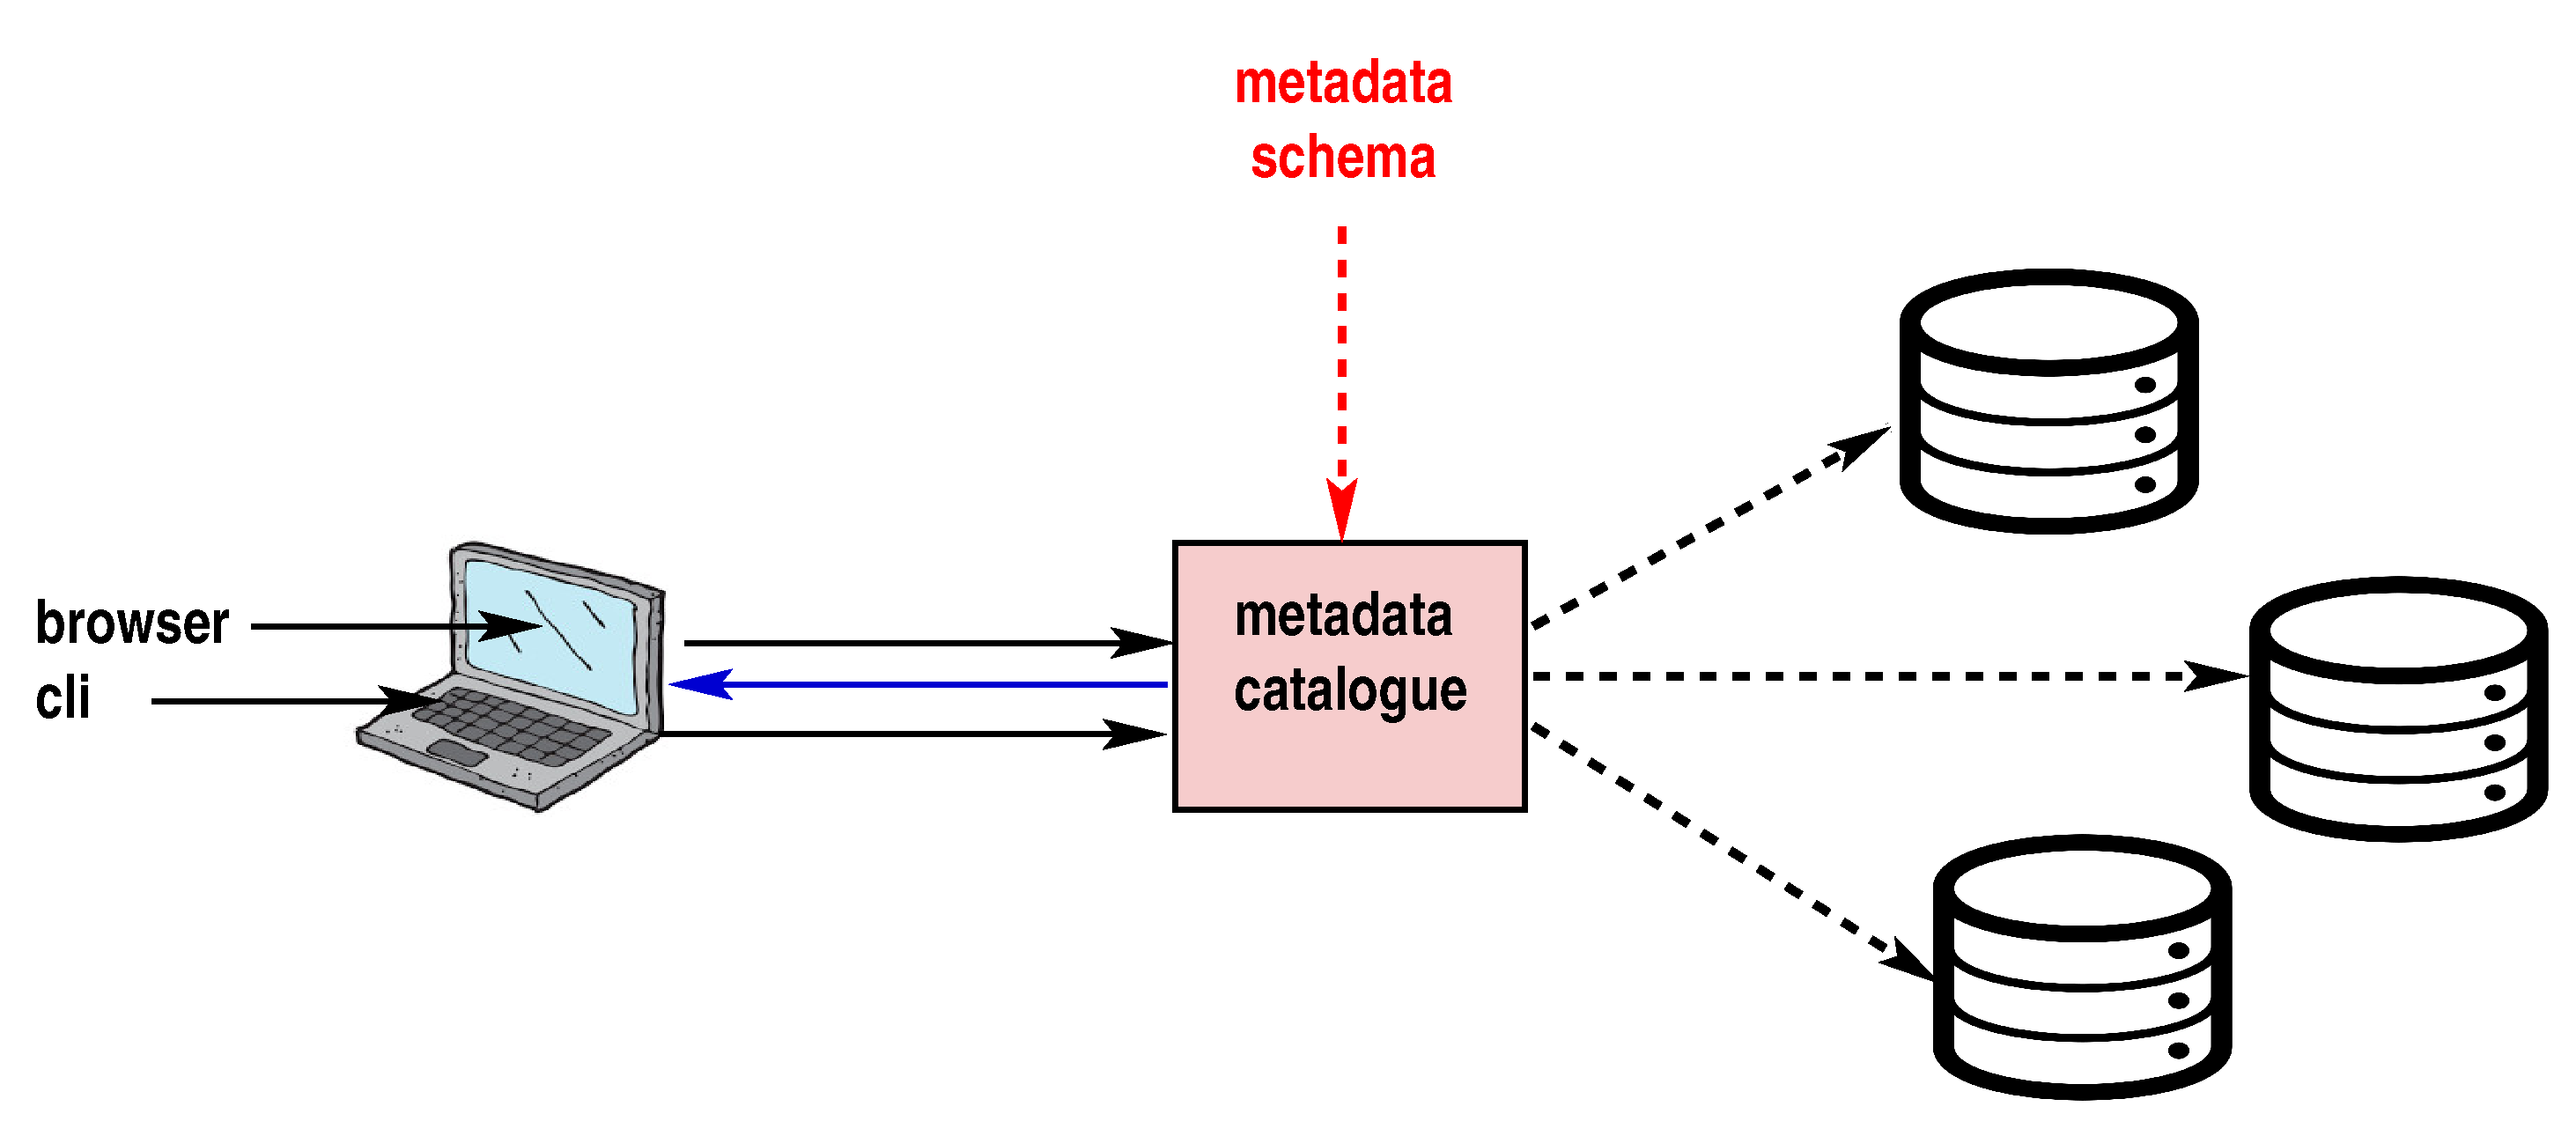
\includegraphics[height=35mm]{\figs/ildg-access1schema}
  \end{center}
    
  Not (just) web pages!
  \bi
  \item grid (or cloud) storage elements (SE)
  \item central Metadata Catalogue(s) (MDC)
  \ei

  
\end{frame}
%------------------------------------------------
\begin{frame}{Global Services and Organization of ILDG}
  \vspace*{3mm}
  \begin{columns}[c]
    \column{0.6\textwidth} 
    ILDG operates only \alert{2 global services}
    \begin{itemize}
    \item VO registration (\href{https://grid-voms.desy.de:8443/voms/ildg}{\green VOMS}) \\[1mm]
      {\small
        registry of ILDG users (groups and roles)\\
        used for authentication to storage elements
        }
    \item Web page (\href{https://hpc.desy.de/ildg}{\green temporary})\\[1mm]
      {\small 
        specification of standards and conventions\\
        URLs of services of each regional grid ({\tt Services.xml})
      }
    \end{itemize}

    \vspace*{5mm}
%%%     Organization
%%%     \begin{itemize}
%%%     \item Board 
%%%     \item Metadata Working Group (MDWG)
%%%     \item Middleware Working Group (MWWG)
%%%     \end{itemize}
%%%     
    \column{0.35\textwidth}
    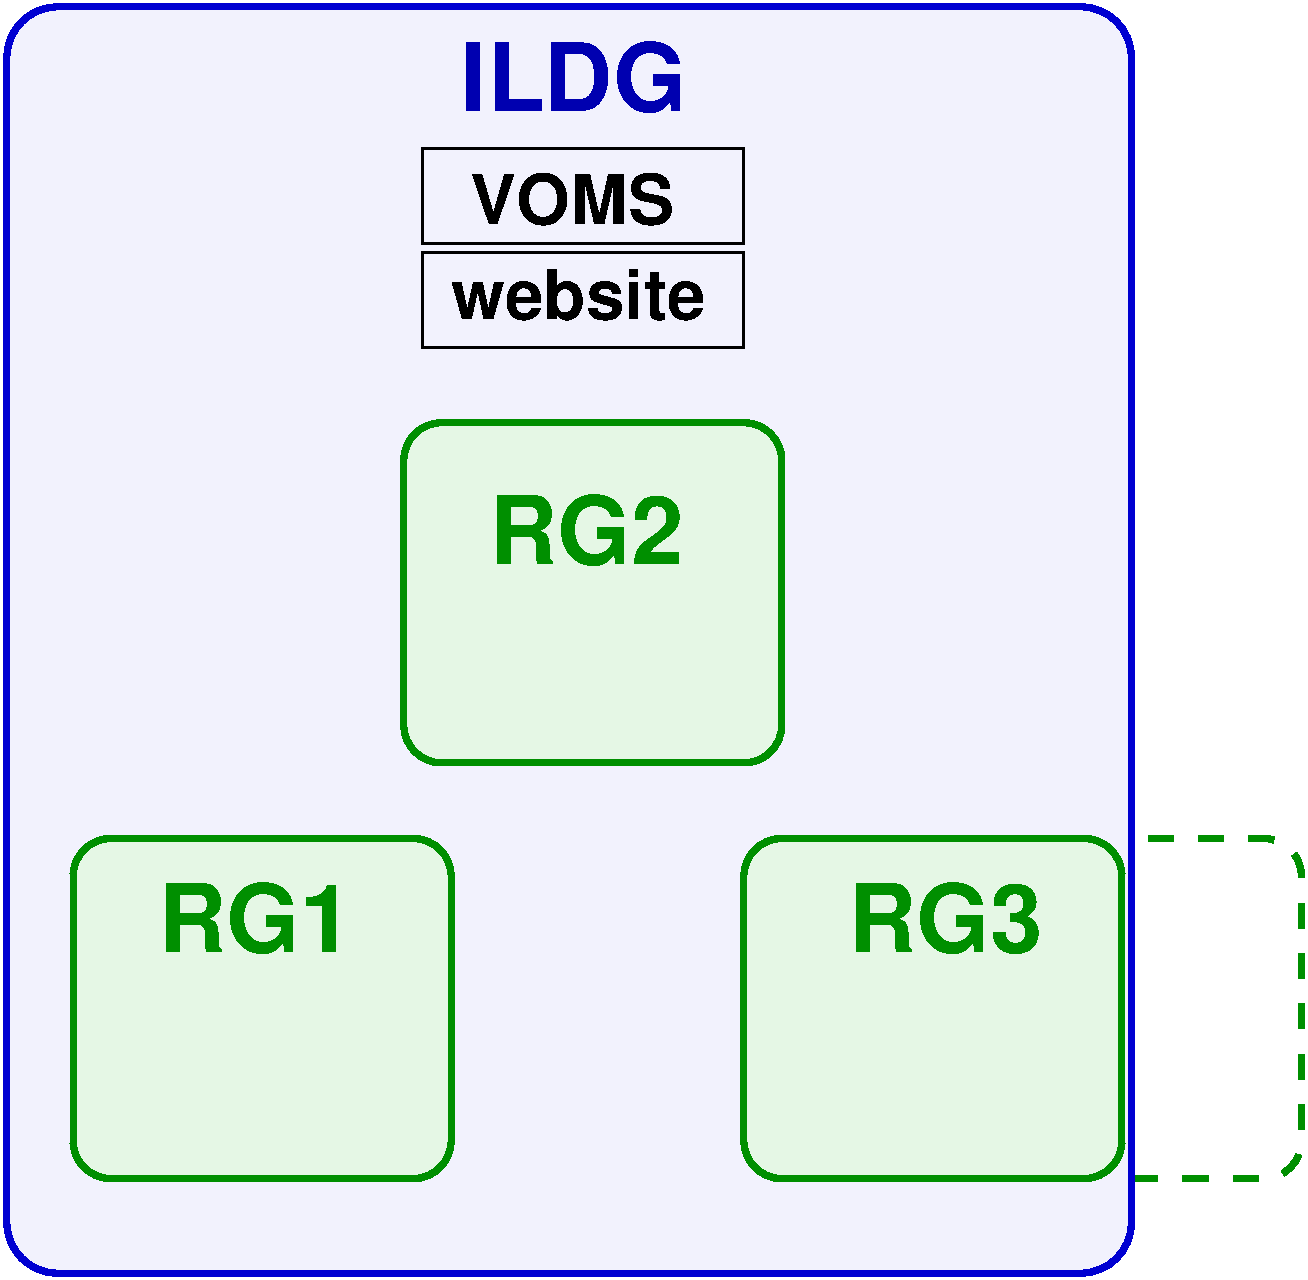
\includegraphics[width=40mm]{\figs/arch-ildg-rg}
  \end{columns}

\end{frame}
%------------------------------------------------
\begin{frame}{ILDG Web Page}
  
  \begin{columns}
    \column{0.45\textwidth}
    \bi
    \item Under construction!
    \item VO Policy
    \item Specifications:
      \bi
      \item metadata schema
      \item file formats
      \item working groups
      \item URLs of services
      \ei
    \item (Incomplete) user documentation
    \ei

    \column{0.45\textwidth}
    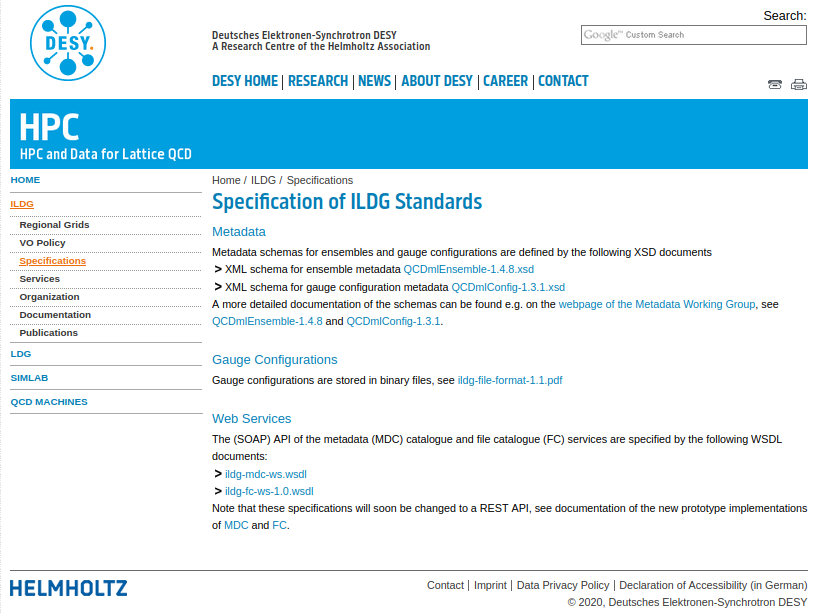
\includegraphics[height=40mm]{\figs/screen-webpage}
  \end{columns}
  
\end{frame}
%------------------------------------------------
\begin{frame}{Membership of the Virtual Organization ``ILDG''}

  \begin{center}
    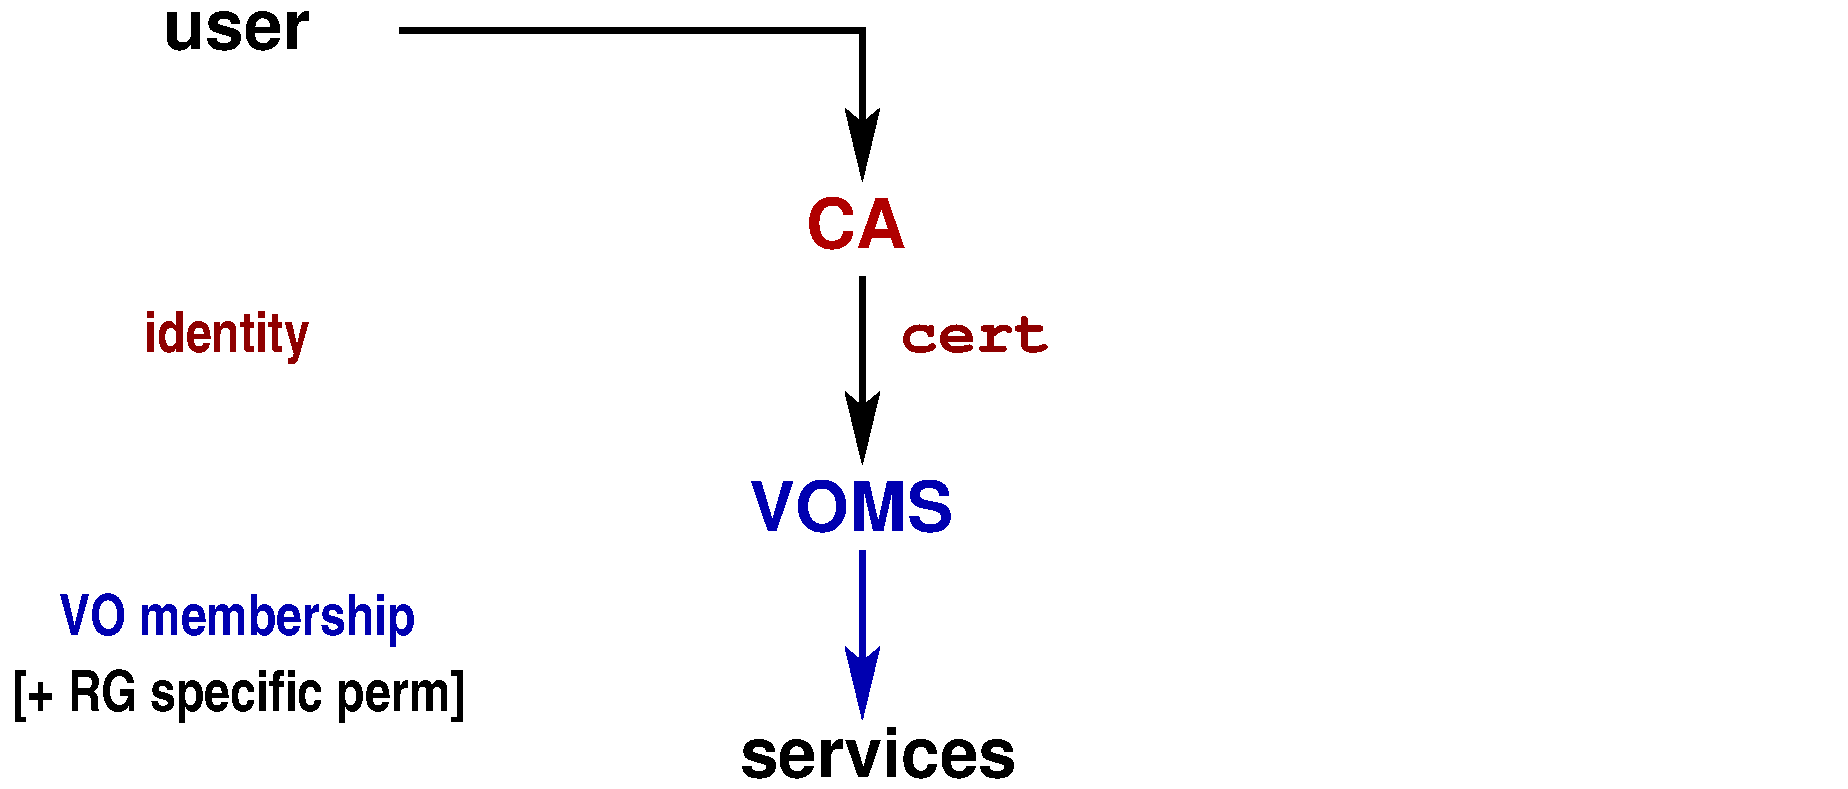
\includegraphics[height=35mm]{\figs/voms2iam1}
    \hspace*{-10mm}
    \fbox{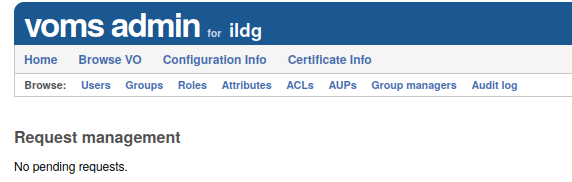
\includegraphics[height=15mm]{\figs/screen-voms}}
  \end{center}

  \vspace*{-3mm}
  Currently: (ILDG 1)
  \bi
  \item identity = grid certificats from \alert{trusted CAs} (\href{https://www.igtf.net/}{IGTF})
  \item membership = \href{https://grid-voms.desy.de:8443/voms/ildg/}{VOMS} hosted at DESY
  \ei

  \vspace*{20mm}

  \vfill
  
\end{frame}
   
\begin{frame}{Membership of the Virtual Organization ``ILDG''}

  \begin{center}
    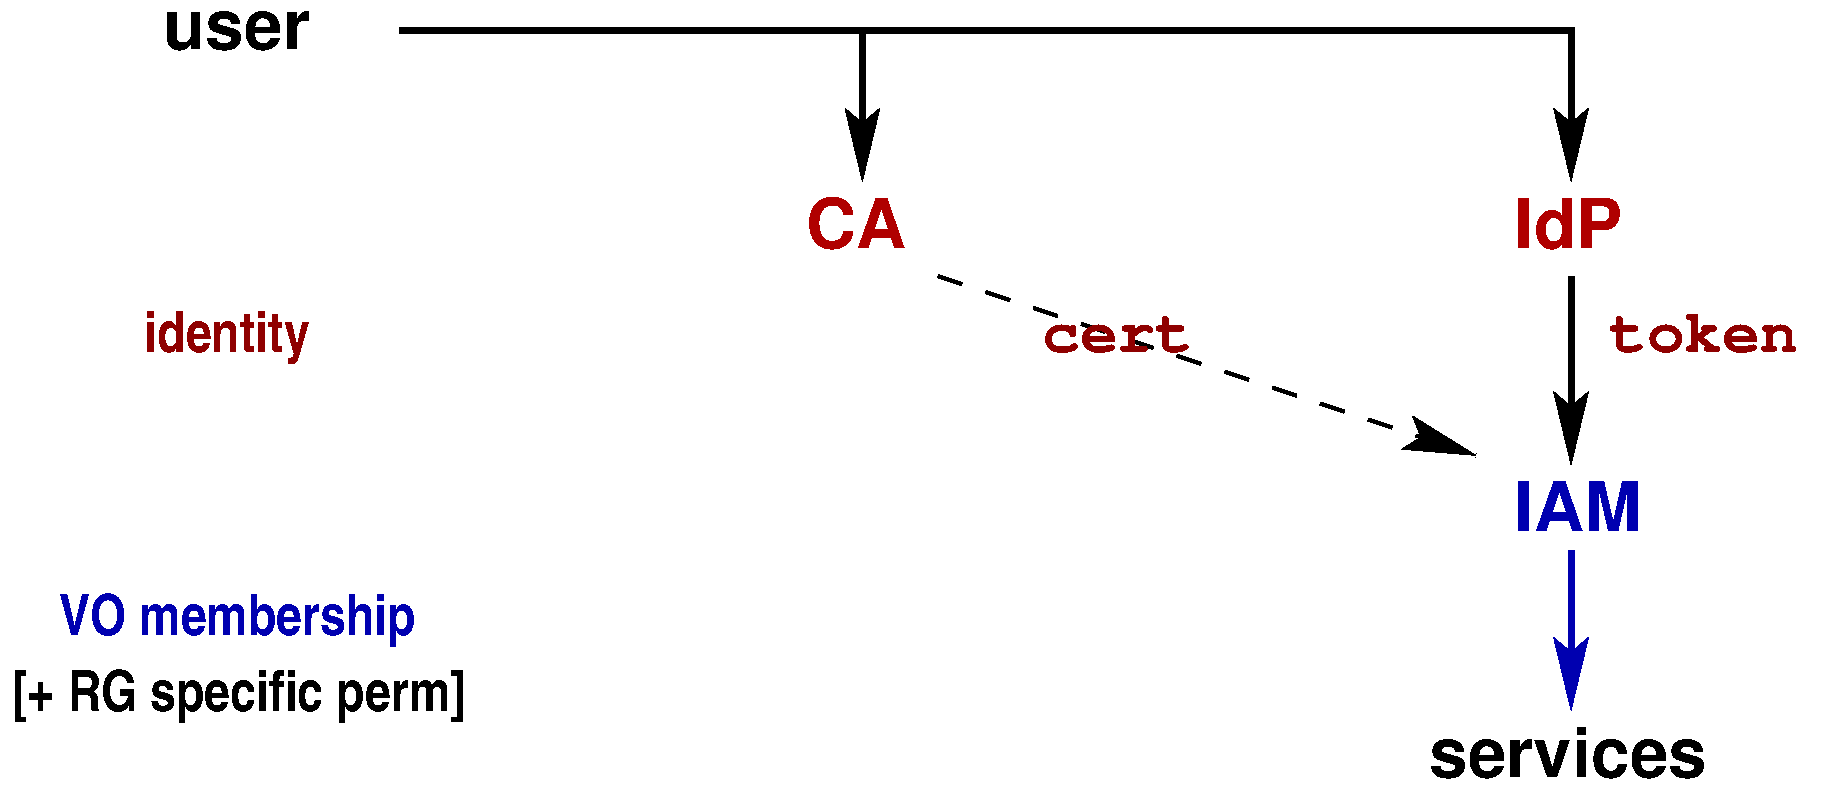
\includegraphics[height=35mm]{\figs/voms2iam2}
    \hspace*{19mm}
    \fbox{
\includegraphics[height=20mm]{\figs/screen-iam}}
  \end{center}

  \vspace*{-3mm}
  Currently: (ILDG 1)
  \bi
  \item identity = grid certificats from \alert{trusted CAs} (\href{https://www.igtf.net/}{IGTF})
  \item membership = \href{https://grid-voms.desy.de:8443/voms/ildg/}{VOMS} hosted at DESY
  \ei

  \vspace*{3mm}
  Future: (ILDG 2)
  \bi
  \item identity = token from \alert{trusted IdPs} (e.g. home institutions in \href{https://technical.edugain.org/}{eduGAIN})
  \item membersiip = IAM (Identity and Access Management) hosted at CNAF/INFN
  \ei

\end{frame}
   
%------------------------------------------------
\begin{frame}{The Need for trusted Identity Proofing}

  Service providers used by ILDG \alert{require a reliable identification} of users, \\
  e.g. for
  \bi
  \item storage (even for read-access only!)
  \item fast (!) network connections
  \ei


%  \vspace*{5mm}
%  \Darrow\ Federations of CAs/IdPs which can guarantee a well-defined \alert{Level of Assurance} (LoA)
%  \begin{center}
%    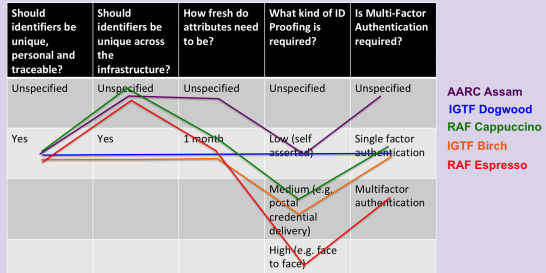
\includegraphics[height=40mm]{\figs/AARC-LoA}
%    \\
%      {\small
%        \href{https://docs.google.com/document/d/1BBJYzSCIGlDrV32w-6vNuSdojIlQMf3ObhsYVgG3P6Q}
%             {AARC Acceptable Authentication Assurance Policy}
%      }
%  \end{center}
  \begin{columns}
    \column{0.40\textwidth}
    \Darrow\ Federations of CAs/IdPs which\\
    \hspace*{5mm} can guarantee a well-defined\\
    \hspace*{5mm}\alert{Level of Assurance} (LoA)

    \vspace*{5mm}
    \Darrow\ Users need to respect rules\\
    \hspace*{5mm} AUP: SPs $\leftrightarrow$ users\\
    \hspace*{5mm} VO Policy: users $\leftrightarrow$ users

    \column{0.55\textwidth}
    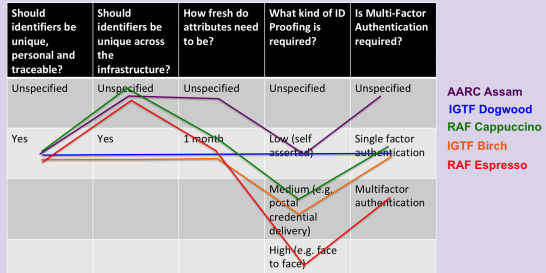
\includegraphics[height=42mm]{\figs/AARC-LoA}
    \\
      {\small
        \href{https://docs.google.com/document/d/1BBJYzSCIGlDrV32w-6vNuSdojIlQMf3ObhsYVgG3P6Q}
             {AARC Acceptable Authentication Assurance Policy}
      }
  \end{columns}

  \vfill
\end{frame}
%------------------------------------------------
\begin{frame}{Autonomous Regional Grids}

  \begin{block}{Services operated by each Regional Grid}
    \begin{itemize}
    \item Metadata Catalog (MDC)
    \item File Catalog (FC)
    \item Storage Elements (SE)
    \item Website with RG-specific information
    \end{itemize}
  \end{block}

  \vspace*{5mm}
   Regional Grids: CSSM, JLDG, LDG, UKQCD, USQCD
    \begin{itemize}
    \item are implemented with different architectures and technologies
    \item operate in an autonomous way with individual policies
    \end{itemize}

    Examples
    \begin{itemize}
    \item JDLG: single SE, no specific access control
    \item LDG: multiple SE, fine grained access control
    \end{itemize}

\end{frame}

%------------------------------------------------
\begin{frame}{JLDG Architecture}

  \begin{columns}[c]  
    \column{0.5\textwidth}
    \begin{itemize}
    \item Single federated storage system (GFARM)
    \item JLDG-internal write access
    \item Fast read access ({\tt gridftp}) available\\
          for VO members
    \item Transition to token-based authentication
    \end{itemize}
    \vspace*{20mm}
    
    \column{0.55\textwidth}
    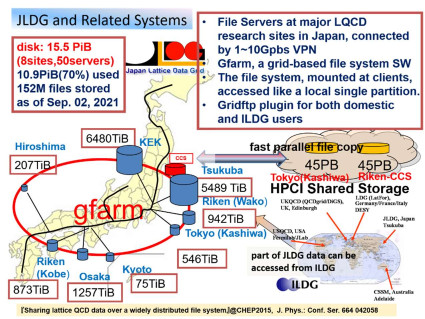
\includegraphics[height=60mm]{\figs/ILDG-perspectives-tomoteru-fig.jpg}
    \\
    \footnotesize{\centerline{T. Yoshie}}
  \end{columns}
  
\end{frame}
%------------------------------------------------
\begin{frame}{USQCD Ideas}
  \begin{center}
    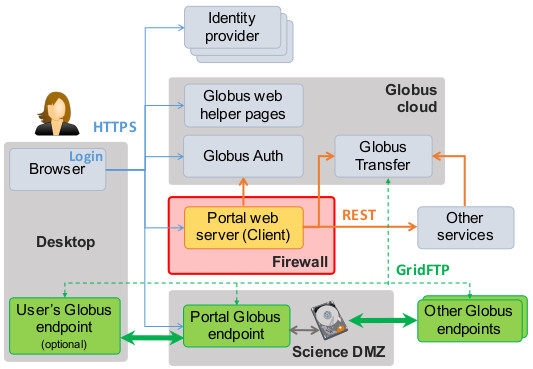
\includegraphics[height=0.7\textheight]{\figs/peerj-cs-144-fig3.jpg}
    \\
    \footnotesize{\href{https://doi.org/10.7717/peerjcs.144/fig-3}{K. Chard et al. 2017}}
  \end{center}

\end{frame}

%================================================
\section{Basic ILDG Services}
%------------------------------------------------
\begin{frame}{Interplay between ILDG Services}
  \begin{center}
    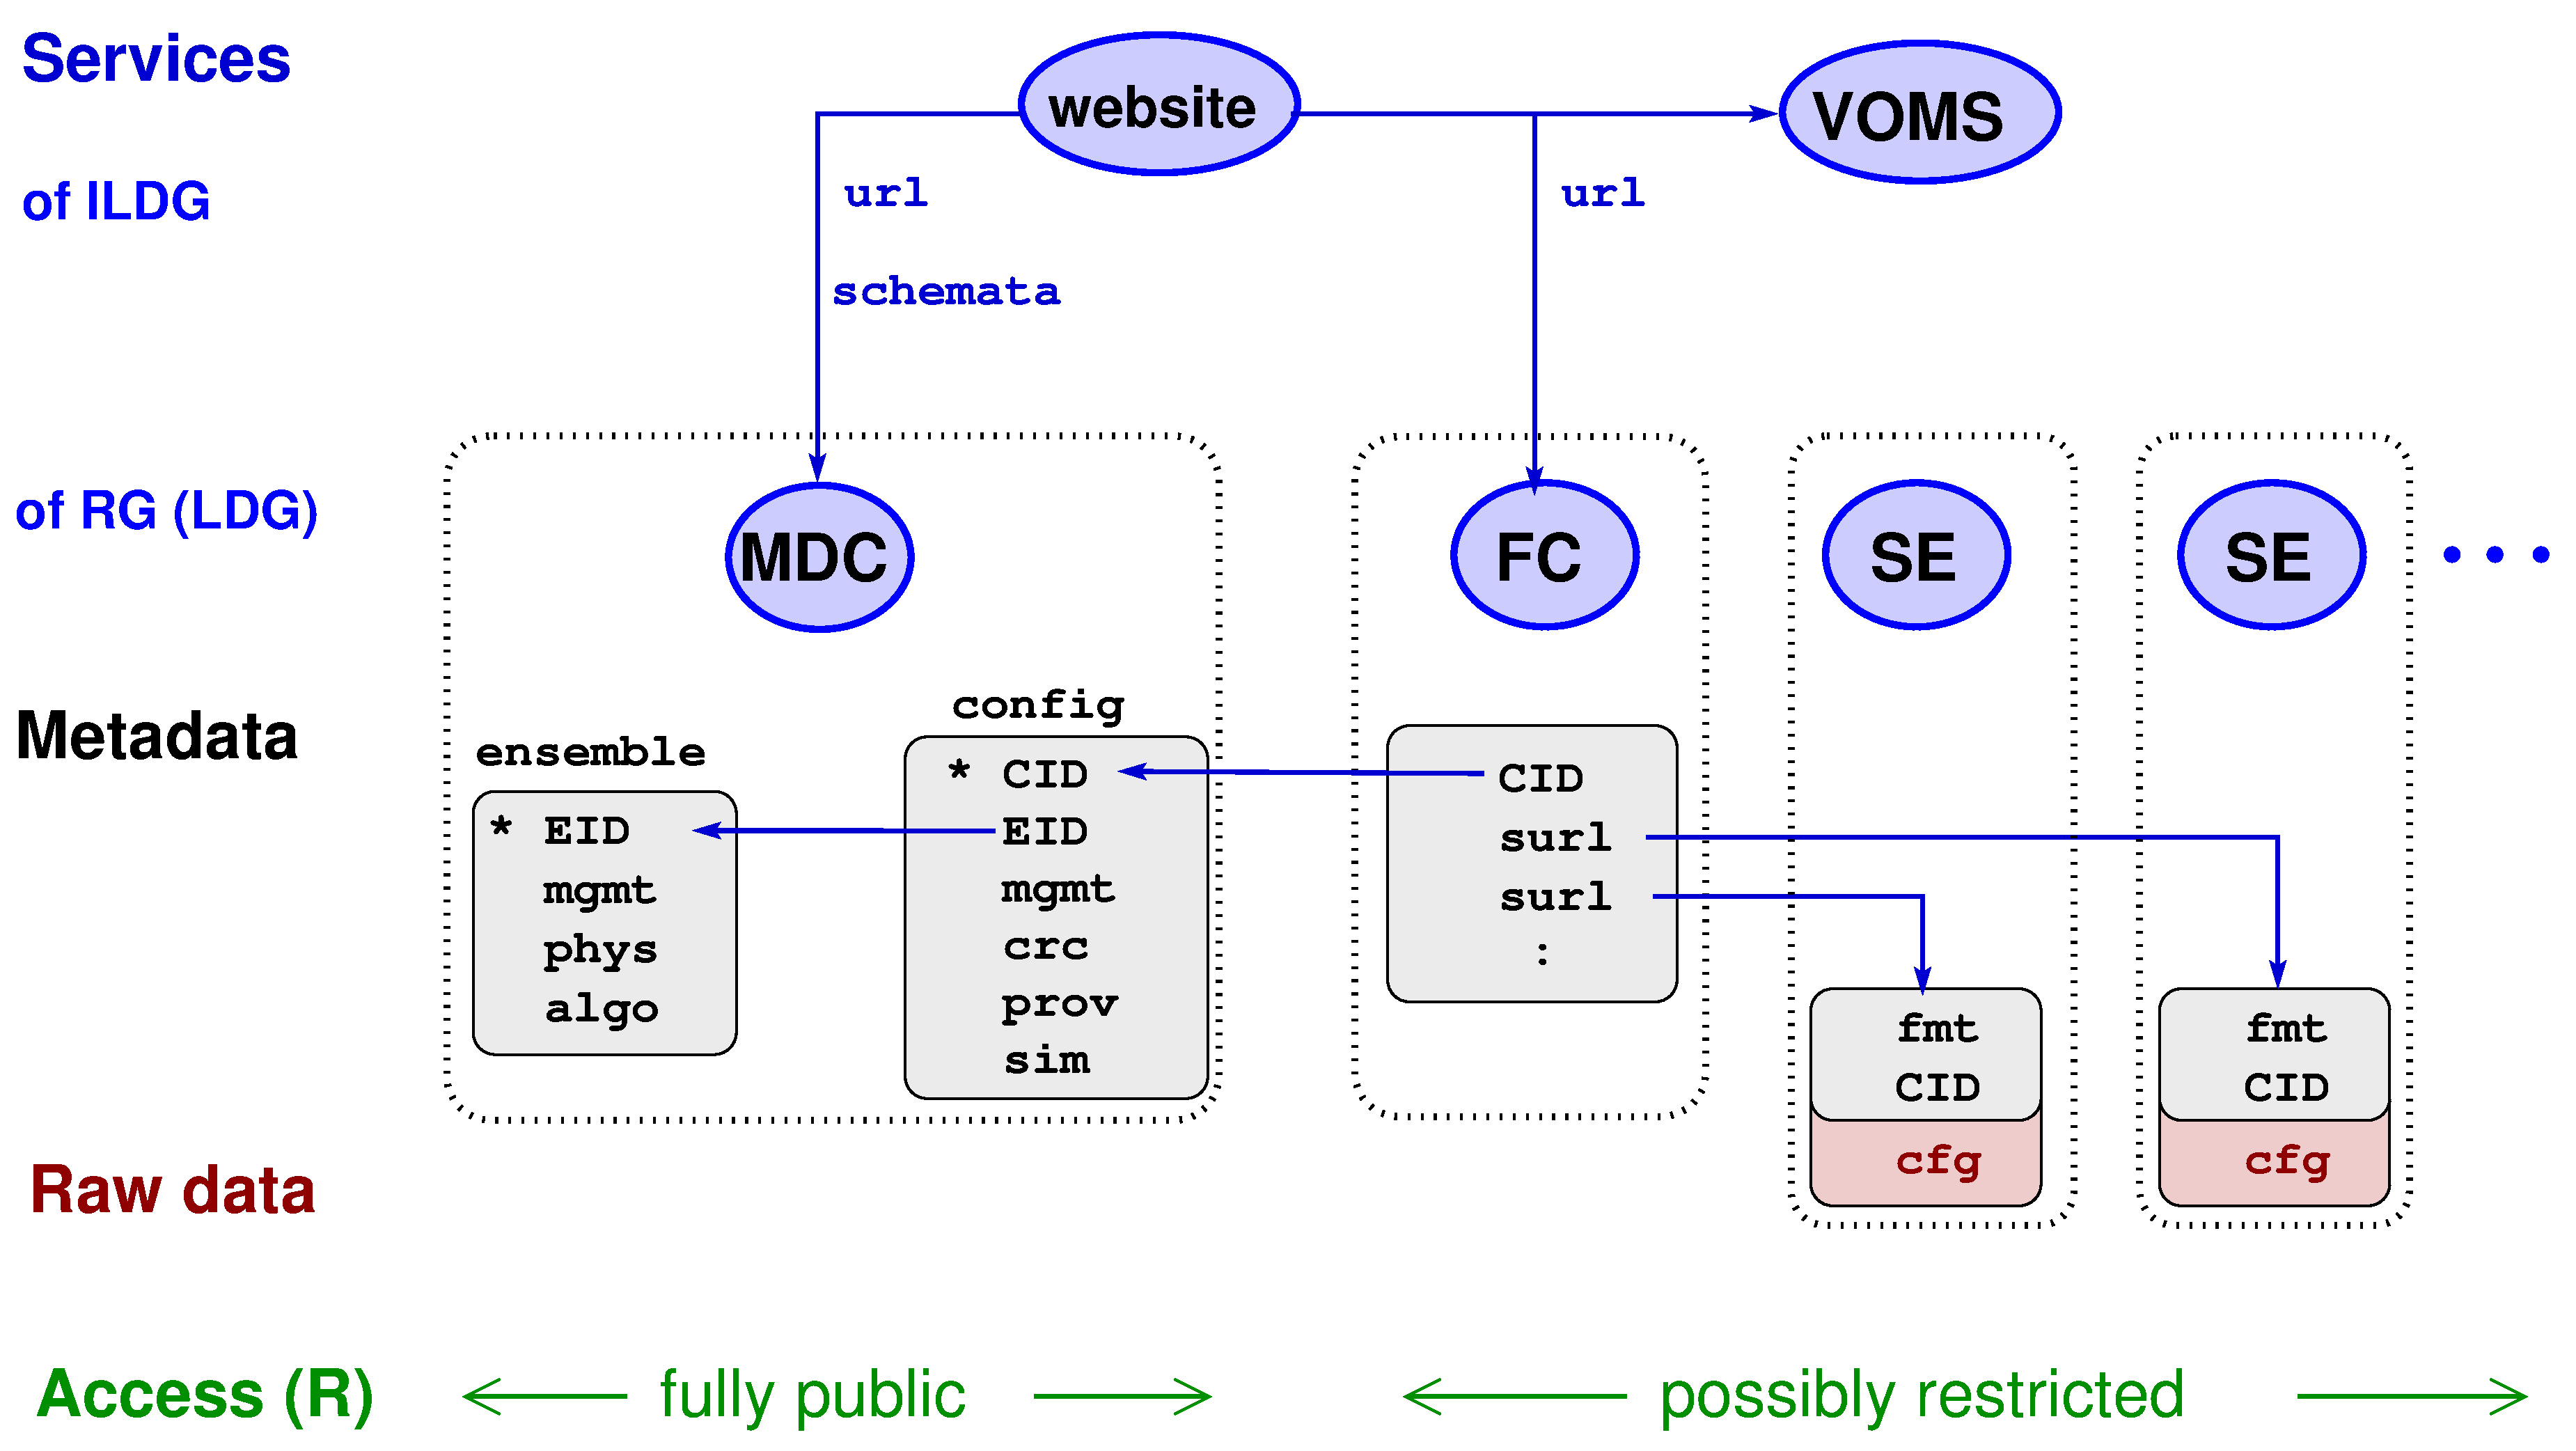
\includegraphics[height=0.8\textheight]{\figs/arch-ildg-db}
  \end{center}

\end{frame}

%------------------------------------------------
\begin{frame}{Metadata Catalogue (MDC)}

  {\bf Key purpose:} ID regisration and metadata search
  \begin{center}
        \fbox{ID $\longleftrightarrow$ metadata}
  \end{center}
  
  {\bf Database schema}
  \begin{center}
    {\small
      \begin{tabular}{l|l|l|l}
                      & \multicolumn{3}{c}{metadata collection name} \\
                      & config         & ensemble             & publication (?) \ldots\\
        \hline 
        primary key:  & LFN (dataLFN)  & MCU (markovChainURI) & DOI (?)    \\
        attributes:   & QCDml tree     & QCDml tree           & t.b.d.     \\
                      & MCU            & license (not yet)    & list of MCU \\
                      &                &                      & DataCite metadata
      \end{tabular}
    }
  \end{center}
  
  {\bf Basic operations}
  \bi
  \item[$\green\ast$] \parbox{14em}{\green Search: query $\to$ list of IDs} (supporting powerful Xpath queries)  \hfill {\bf F4}
  \item[$\green\ast$] \parbox{14em}{\green Retrieve: ID $\to$ MD} (QCDml schema)                                 \hfill {\bf A1}
  \item Validate, insert, update, delete, \ldots
  \ei
  
\end{frame}
%------------------------------------------------
\begin{frame}{File Catalogue (FC)}

  {\bf Provides:} functional (many-to-one) relation 
  \begin{center}
    \fbox{FC: SURL $\longrightarrow$ LFN}
  \end{center}
  
  {\bf Database schema}
  \begin{center}
    \begin{tabular}{ll}
      primary key: & SURL (Storage URL)\\
      attributes:  & LFN  \\
      & MCU  {\small (or other optional Access Control Attributes)}
    \end{tabular}
  \end{center}
  
  {\bf Basic operations}
  \bi
  \item[$\green\ast$] {\green list entries (SURL) by LFN}          \hfill {\bf A1}
  \item list by other criteria (SURL, Access Control Attributes)
  \item insert, update, delete, \ldots
  \ei

\end{frame}
%------------------------------------------------
\begin{frame}{New Implementation of MDC and FC}

  \vspace*{-5mm}
  \hfill 
\includegraphics[height=17mm]{figs1/PUNCH4NFDI-Logo_RGB.jpg}

  \vspace*{-22mm}
  \begin{center}
    (by Basavaraja BS $@$ DESY/NIC)
  \end{center}
  
  {\bf Technical details} 
  \bi % \vspace*{-2mm}\setlength{\itemsep}{-1mm}
  \item configurable, e.g. for additional collections (beyond ensembles and configs)
  \item additional attribute service for access control (ACS)
  \item REST API (see online documentation
    \href{https://idefix-vm10.zeuthen.desy.de/ildg/mdc/swagger-ui/index.html}{MDC},
    \href{https://idefix-vm10.zeuthen.desy.de/ildg/fc/swagger-ui/index.html}{FC}, and
    \href{https://idefix-vm10.zeuthen.desy.de/ildg/acs/swagger-ui/index.html}{ACS})
  \item simple deployment (Docker containers, Kubernetes in preparation)\\
    e.g. for other regional grids or applications
    \bi
    \item[$\green\bullet$] JLDG: 60 ensembles, 40 k configs \\
    \item[$\green\bullet$] LDG: 2 instances, 250 ensembles, 250 k configs (not yet consistent with SE)
    \item[$\blue\bullet$] UK: in preparation
    \ei
  \ei
  \vfill
\end{frame}
%================================================
\section{Interacting with ILDG Services}
%------------------------------------------------
\begin{frame}{Interaction with ILDG Services}

  \begin{center}
    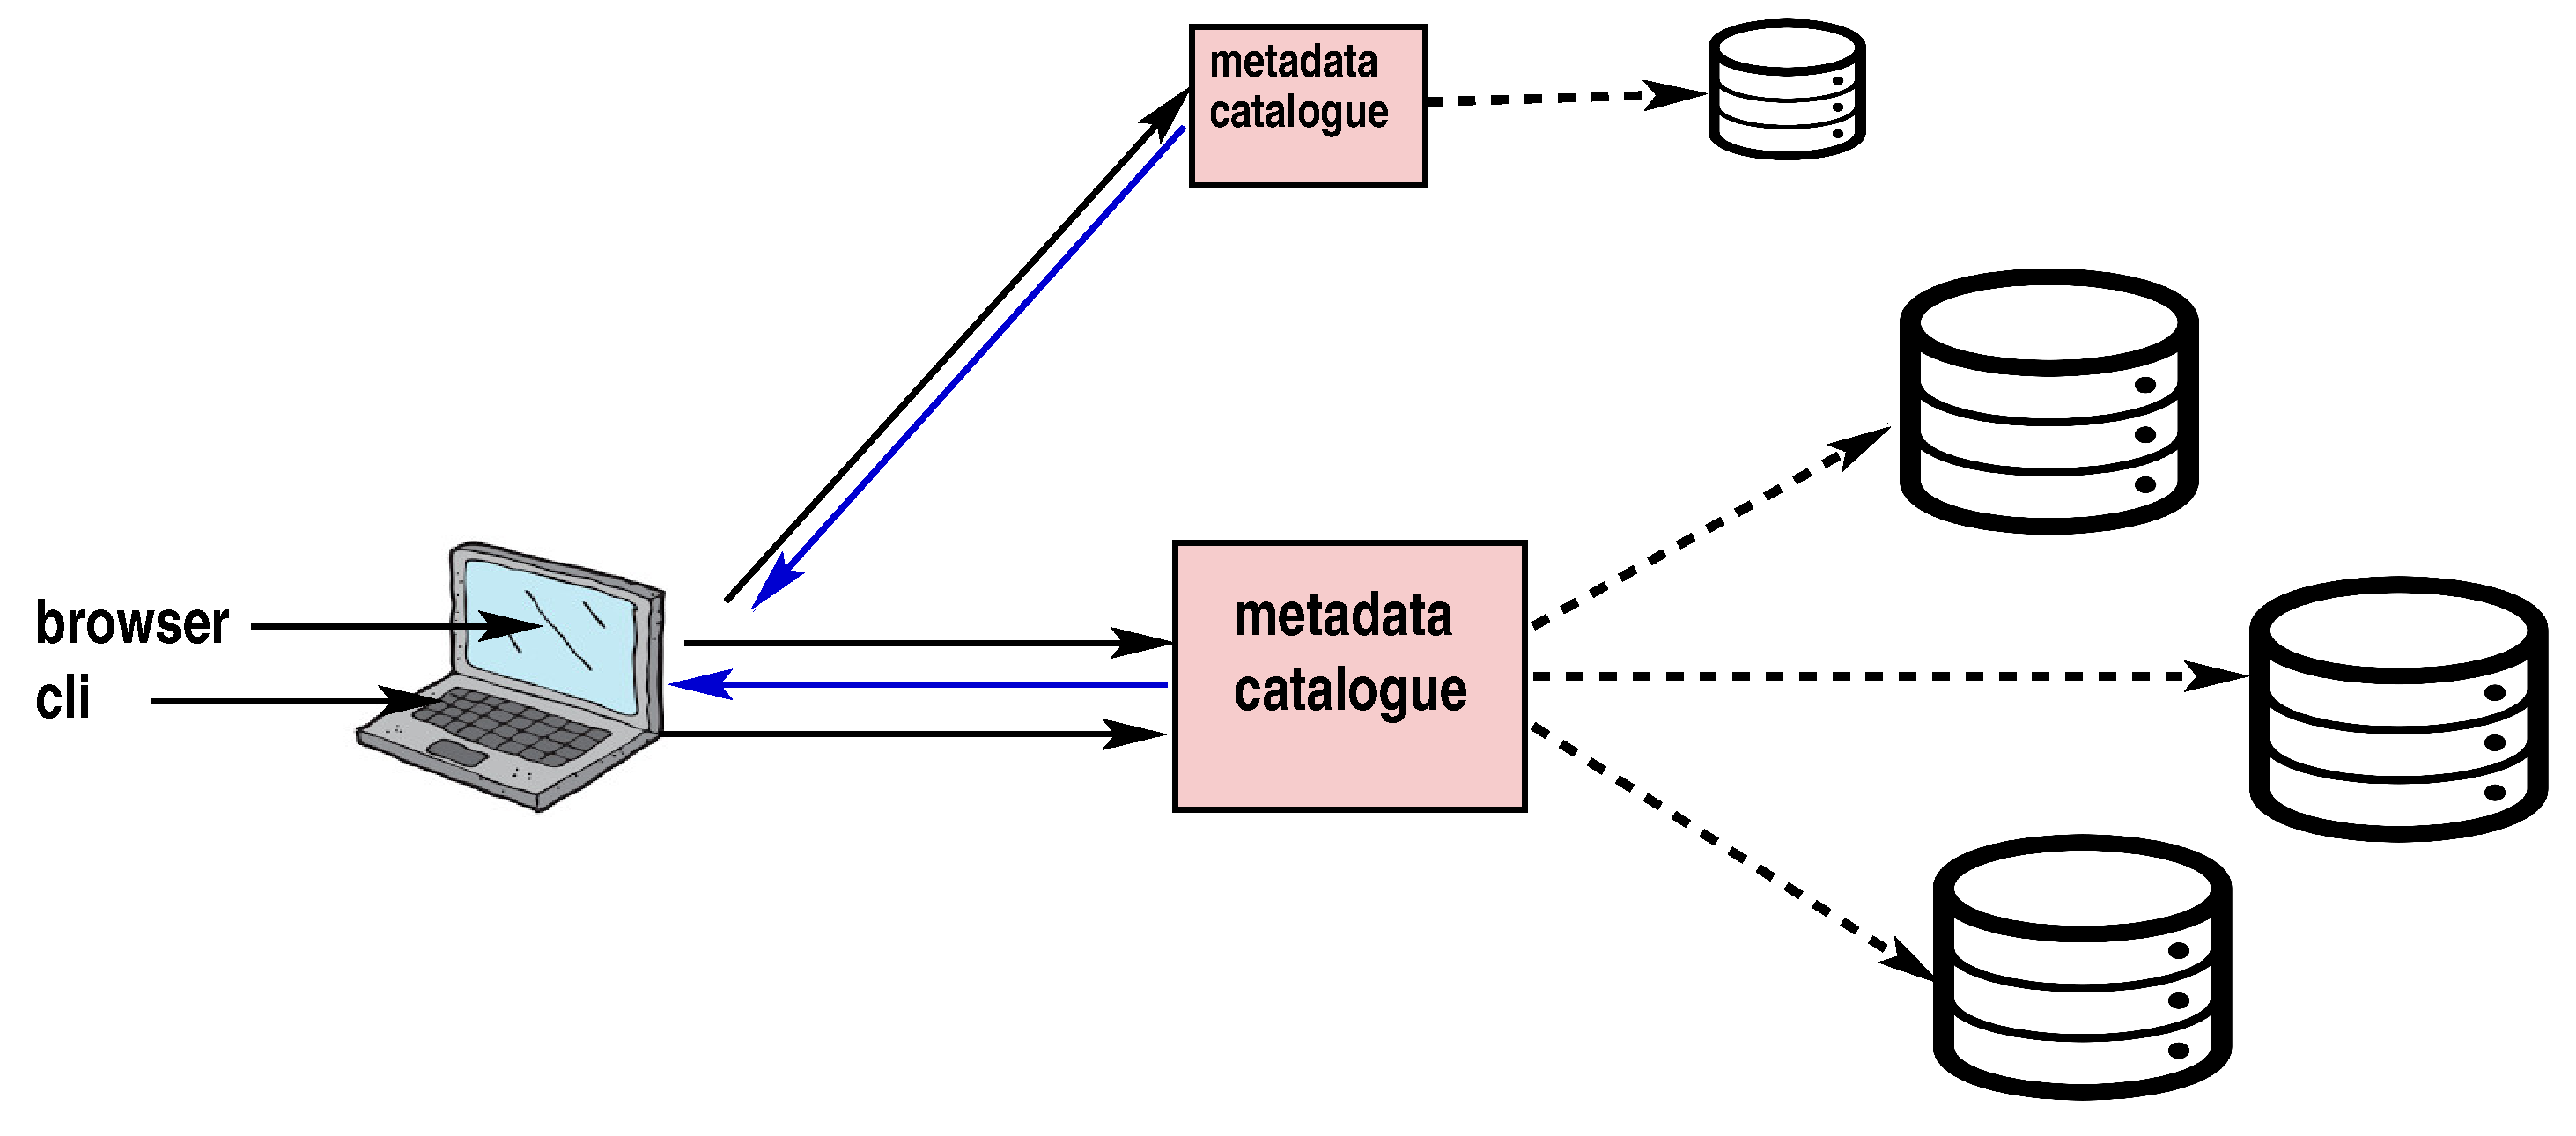
\includegraphics[height=35mm]{\figs/ildg-access2}
  \end{center}

  \begin{dinglist}{114}
    \item Catalogues of all regional grids are \alert{interoperable} due to standardized API

    \item  High-level user operations may need several ($\le 10$) low-level requests (e.g. HTTP)\\
      but still few compared to other web pages (implicitly handled by your browser)
      \bi
    \item www.google.com: O(25) requests 
    \item www.github.com: O(100) requests \hspace*{20mm} (try Ctrl-Shift-I in firefox)
    \item your favourite airline: O(200) requests
      \ei
  \end{dinglist}
  \vfill
\end{frame}
%------------------------------------------------
\begin{frame}{Consistency of ILDG Data}
  \begin{dinglist}{114}
    \item ILDG is logically a distributed relational database with 2 kinds of entities
      \bi
    \item configs: metadata + (binary) data
    \item ensembles: metadata
    \ei
    and corresponding primary keys
    \bi
    \item \parbox{12em}{LFN (dataLFN):} \alert{\tt lfn://{\it rg}/{\it collaboration}/{\it project}/{\it name}}
    \item \parbox{12em}{MCU (markovChainURI):} \alert{\tt mc://{\it rg}/{\it collaboration}/{\it project}}
    \ei

  \item[\ding{42}] Persistence and globally unique identifiers needs to be guaranteed by data providers.
  
  \item Typical inconsistencies (RDB anomalies) may arise from
  \bi
  \item failures of individual services
  \item incorrect use of low-level tools
  \ei
  and can only be
  \bi
  \item detected and fixed by regular scans (with possibly prohibitive cost)
  \item checked and handled by high-level tools (including roll-back)
  \ei
  \end{dinglist}
  \vfill
\end{frame}
%------------------------------------------------
\begin{frame}{Use Cases and  ``ltools''}
\def\lcol{0.45\textwidth}
\def\rcol{0.5\textwidth}

\begin{columns}  
    \column{\lcol}
    Consumer (collaboration internal)
    \begin{itemize}
    \item \alert{\tt lfind}: search in metadata catalog
    \item \alert{\tt lget}: download data and metadata
    \end{itemize}
    \vspace*{3mm}
    
    \column{\rcol}
    Provider (collaboration internal)
    \begin{itemize}
    \item \alert{\tt lpack}: generate markup${}^{*)}$ and pack data
    \item \alert{\tt linit}: register ensemble metadata 
    \item \alert{\tt lput}: upload config data and metadata
    \end{itemize}
  \end{columns}

  \vspace*{3mm}
  \begin{columns}  
    \column{\lcol}
    \centerline{$\downarrow$}
    \column{\rcol}
    \centerline{$\downarrow$}
  \end{columns}
  
  \vspace*{5mm}

  \begin{columns}  
    \column{\lcol}
    Consumer (community wide)
    \begin{itemize}
    % \item same as collaboration internal
    \item optionally also use common search\\
      engines
    \item cite DOIs when using published data
    \end{itemize}
    
    \column{\rcol}
    Provider (community wide)
    \begin{itemize}
    % \item same as collaboration internal
    \item optionally register DOI and\\
      generate landing page
    \item drop access restriction flag
    \item receive data citation record
    \end{itemize}
  \end{columns}

  \vspace*{5mm}
  \begin{columns}  
    \column{\lcol}
    ~
    \column{\rcol}
           {\small \parbox{2em}{\hfill ${}^{*)}$} trivial if information is already\\
             \parbox{2em}{~} collected during production!}
  \end{columns}

\end{frame}
%------------------------------------------------
\begin{frame}{Examples of Interactions with ILDG Services}

  \begin{dinglist}{114} \setlength{\itemsep}{2mm}
    \item ``Login'' to ILDG: {\tt voms-proxy-init}
      \bi
      \item periodically ($\le$ 2 days) download latest CRLs \hfill $\longleftrightarrow$ \parbox{4em}{CA}$~$ \parbox{4em}{~}
      \item unlock your private key (by pass phrase) \\[-1mm]
        or login at your IdP                                 \hfill $\longleftrightarrow$ \parbox{4em}{~}$~$ \parbox{4em}{IdP}
      \item request VO membership info and attributes        \hfill $\longleftrightarrow$ \parbox{4em}{VOMS}$\vert$ \parbox{4em}{IAM}
      \item generate VOMS proxy 
      \ei
    \item ``Get'' config data (for specific and known LFN)
      \bi
      \item optionally download config (and ensemble) metadata  \hfill $\longleftrightarrow$ \parbox{8em}{MDC}
      \item authenticate with proxy to FC and request SURL list \hfill $\longleftrightarrow$ \parbox{8em}{FC/AC}
      \item authenticate to SE and download data                \hfill $\longleftrightarrow$ \parbox{8em}{SE/AC}
      \ei
    \item ``Put'' config data (for existing ensemble)
      \bi
      \item upload config metadata                              \hfill $\longleftrightarrow$ \parbox{8em}{MDC/AC}
      \item decide SE and SURL (agreed with RG admin)
      \item register SURL                                       \hfill $\longleftrightarrow$ \parbox{8em}{FC/AC}
      \item upload binary                                       \hfill $\longleftrightarrow$ \parbox{8em}{FC/AC}
      \ei  
  \end{dinglist}
  \vfill
\end{frame}

%------------------------------------------------
\begin{frame}{Hands-on Exercises}

  Please keep in mind:
  
  \begin{dinglist}{114}

  \item you are using a prototype system, some components of which have\\
    been re-activated or newly developed only during the last months
    
  \item currently we do not (yet/any more ) have user-friendly ``ltools'',\\
    but only quick and dirty scripts for low-level operations:
    \bi
    \item {\tt try-mdc}, {\tt try-fc}, {\tt try-acs} (just wrapper scripts for {\tt curl})
    \item {\tt lime-ls}, {\tt lime-cat1}, {\tt lime-pack1}
    \item {\tt ildg-cksum}, {\tt ildg-binary}
    %%% \item {\tt md-convert}
    \ei

    \ldots\ you all can improve them and contribute to develop proper user tools!
  \end{dinglist}

  \vfill
\end{frame}
%------------------------------------------------
\begin{frame}{Hands-on Exercises (cont.)}
  \begin{dinglist}{114}
  \item Required SW packages are installed in the workshop image (docker + apptainer)\\
    which you should have running according to the
    \href{https://gitlab.desy.de/ildg/hands-on/workshop-image/blob/main/README.md}{instructions} . \\
    {\small
      In particular, the container includes
      \bi
      \item {\tt voms-proxy-init}
      \item {\tt gfal} commands
        (\href{http://grid-deployment.web.cern.ch/grid-deployment/dms/dmc/docs/gfal2-2.10.2/}{Grid File Access Library})
      \item {\tt curl} (version working with proxy certificates) and other utilities
      \ei
    }
  \item Additional material is on \href{https://gitlab.desy.de/ildg/hands-on}{gitlab}
   \bi
   \item \href{https://gitlab.desy.de/ildg/hands-on/material.git}{exercise instructions}
   \item \href{https://gitlab.desy.de/ildg/hands-on/try-client.git}{scripts for low-level testing ({\tt try-*})}
   \ei
  \item Ready to get hands on? (and fingers dirty!)

  \item Please also prepare 1 slide/group for the wrap-up discussion on Friday \\
    {\small
      \bi
      \item Which technical aspects did not work or are difficult / inconvenient?
      \item Which technical aspects worked well or are convenient?
      \item Which aspects of the markup are problematic for your project?
      \item Which elements of the metadata schema are missing / incompatible for your projects?
   \ei
    }
  \end{dinglist}
  \vfill
\end{frame}
%------------------------------------------------
% \begin{frame}{Command-line tools}
%   \begin{tabular}{ll}
%     \tt {lls}   [-g <grid>]     & list all ensembles          (of specified RG) \\
%     \tt lls   <uri>		      & list configs of ensemble {\tt <uri>} \\
%     ~\\
%     \tt {lfind} [-g <grid>] -e <xpath>  & Xpath search in ensemble MD (of specified RG) \\
%     \tt lfind [-g <grid>] -c <xpath>  & Xpath search in config MD   (of specified RG) \\
%     ~\\
%     \tt {lget}  <uri>	      & download MD of ensemble {\tt <uri>}  \\
%     \tt lget  <lfn>		      & download MD of config {\tt <lfn>}    \\
%     \tt lget	-d <lfn>	      & download data of config {\tt <lfn>}  \\
%                                       & \\
%     \hline
%     \tt linit  ...		      & register new ensemble \\
%     \tt {lput} ...	      & upload ... \\
%     \tt ladm  ...		      & manage access control \\
%   \end{tabular}
% \end{frame}

\end{document}


